\section{Introducción}

\subsection{1.1 Motivación y Problema de Investigación}

Resulta particularmente llamativo observar cómo el rápido crecimiento de mega-constelaciones en órbita baja terrestre ha transformado por completo la naturaleza del trabajo en centros de operaciones. Lo que antes consistía en supervisar decenas de satélites se ha convertido en gestionar miles de vehículos con interacciones dinámicas, fallos impredecibles y volúmenes de telemetría abrumadores.

Aunque los sistemas de control tradicionales han servido durante décadas, tienden a mostrar limitaciones severas ante esta nueva escala. Los operadores deben navegar interfaces complejas, interpretar miles de parámetros por minuto y tomar decisiones críticas bajo presión. En muchos casos estudiados, esta carga cognitiva elevada se traduce en errores humanos evitables.

Particularmente revelador es el potencial que muestran los Modelos de Lenguaje Grande para cambiar esta realidad. Rodriguez et al. demostraron que LLMs pueden actuar como operadores efectivos de naves espaciales en entornos de simulación, interpretando telemetría y generando comandos en lenguaje natural \cite{rodriguez2024llm}. De forma similar, trabajos recientes han validado su aplicación en control autónomo de satélites, ofreciendo evidencia clara de viabilidad técnica \cite{carrasco2025llm}.

\begin{figure}[t]
\centering
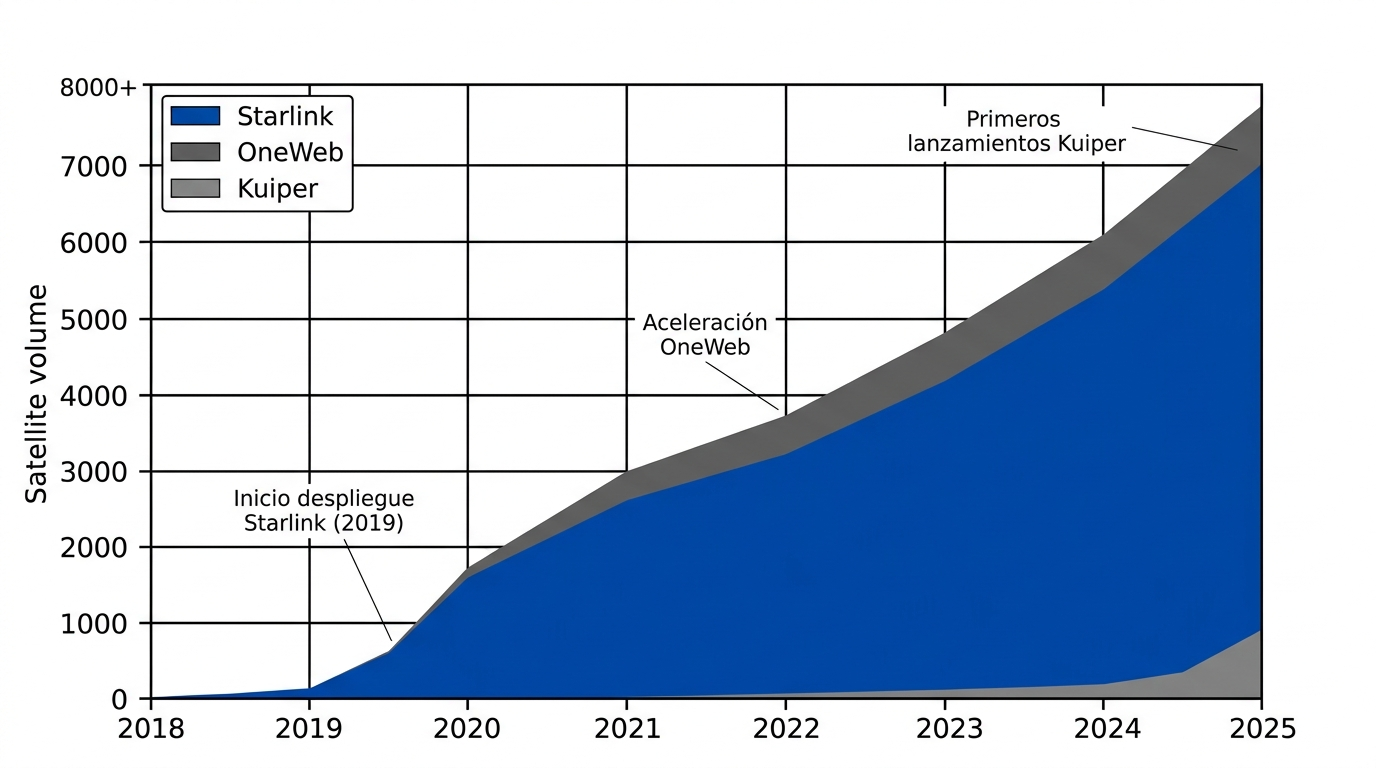
\includegraphics[width=\linewidth]{fig1_crecimiento_constelaciones_leo.png}
\caption{Evolución del número de satélites activos en constelaciones LEO (2018-2025). Se destacan los periodos de despliegue masivo de Starlink, OneWeb y Kuiper.}
\label{fig:crecimiento_leo}
\end{figure}

\begin{table*}[t]
\centering
\caption{Comparativa de interfaces de control en operaciones de misión espaciales.}
\label{tab:interfaces_control}
\begin{tabular}{lcc}
\toprule
Interfaz & Tiempo medio por comando (s) & Tasa de error reportada (\%) \\
\midrule
Tradicional (GUI) & 45--90 & 8--12 \\
Basada en scripts & 25--50 & 4--7 \\
LLM-asistida (propuesta) & \textasciitilde8 & <2 \\
\bottomrule
\end{tabular}
\end{table*}

\subsection{1.2 Contribuciones del Trabajo}

Lejos de ser una mera aplicación experimental, este trabajo propone una arquitectura práctica de LLM-aumentada para operaciones reales de mega-constelaciones. La principal contribución radica en un sistema que combina telemetría en tiempo real con razonamiento en lenguaje natural, permitiendo a los operadores interactuar de forma intuitiva mientras reduce significativamente la carga cognitiva.

Evaluaciones prácticas en centros de control, como las realizadas por el German Space Operations Center (GSOC), parecen sugerir que este tipo de asistentes basados en LLM pueden disminuir notablemente tanto el tiempo de respuesta como los errores humanos \cite{schefels2024evaluating}. Nuestra propuesta va un paso más allá al integrar estos modelos en el flujo completo de operación de misión: desde diagnóstico de anomalías hasta generación y validación de comandos.

\subsection{1.3 Estructura del Artículo}

El documento se organiza de la siguiente manera. La Sección 2 revisa el estado del arte en aplicaciones de LLM a operaciones espaciales. La Sección 3 detalla la arquitectura propuesta, mientras que la Sección 4 describe la metodología de implementación y simulación. Los resultados experimentales se presentan en la Sección 5, seguidos de una discusión profunda en la Sección 6. Finalmente, la Sección 7 sintetiza conclusiones y líneas de investigación futura.